\documentclass[12pt, letterpaper]{article}
\usepackage[utf8]{inputenc}
\usepackage{graphicx}
\usepackage{amsmath}

\title{Creating a Test Statistic to Find if the Number of Misses in a Song from Guitar Hero is Random}
\author{Shannon Coyle, Samantha Colucci, and Brianna Cirillo}
\date{December 2020}

\begin{document}
\maketitle

\section{INTRODUCTION}
The game, Guitar Hero, collects information regarding the number of “hits” recorded by the player.  This poses the question about the randomness of the misses in a song and if they are correlated to the difficulty of the part of the song.

The study investigates the randomness of different songs using varying methods.  These methods looked at the number of miss streaks over the total number of misses, distances between each miss, and using the runs test.  The resampling of the data sets was performed through parametric bootstrapping, permutation tests, and regular bootstrapping. Using resampling and our methods together allowed us to assess the randomness of a given song based on the results. 

This report explains the methodology used in order to test the randomness of a song. The methods and resampling used throughout the project gave results for the empirical type 1 error and the power of the test. These methods were applied to different songs, therefore, returning different results. This report will also look at the limitations and future ideas for the project, and how some of our methods worked well while others did not.

\section{METHODOLOGY}
\subsection{Method 1}
The first method looks at the proportion of the number of miss streaks over the number of total misses.  A streak was definied as one or more misses in a row since it was easier with the code and some samples did not have that many streaks to look at.  From this method, we discovered that the proportion does not tell us anything about the location of the misses.  This proved to be difficult to determine randomness of misses without knowing the exact location of them.  

\subsection{Method 2}
The second method calculates the distances between misses in a song.  The idea behind this method was that if we can see where the misses are occurring, we can see if they are random.  We can seeing where the distances are occuring randomly and conclude that the misses must also be occurring randomly. 

There was an attempt to use a median distance as a basis rather than the mean because the distances were varied, so the average would not tell us that much.  This led to a problem because a lot of the songs had long miss streaks, which lead to a distance of 0, so the median would also become zero.  With this small issue, it led to the idea of use the runs test on this method and, therefore, the distances.  

\subsection{Runs Test}
Knowing that the runs test is a preconceived test for randomness, the idea behind using this was to use it on the distances of misses within a song, rather than just using it on the song. As mentioned previously if a conclusion can be reached that the distances are random, this would imply randomness of the misses in the song. 

A run is defined as a series of increasing or decreasing values, while the number of values in each series is the length of each run. The number of runs in a data set, denoted R, is crucial because this is the number that is used to derive the test statistic. The other values involved in deriving the test statistics is the expected number of runs, denoted $\overline{R}$, the median value of the data sample, the standard deviation of the number of runs, and the number of values below and above the median. 

Once the test statistic is derived, the runs test comes to a conclusion about whether or not to reject the null hypothesis. Here, the test defines: 


The runs test program used was found from the snpar package in RStudio. A p-value, the number of runs and an alternative hypothesis of nonrandomness is produced once the test is run. This package was specifically chosen because was created to be used on discrete data, rather than continuous. When using this method, each song was resampled and a distance vector for each sample was computed. The runs test was then used on the distances to determine if the null hypothesis of randomness should be rejected or not. 

\subsection{Resampling Methods}
\subsubsection{Parametric Bootstrap}
The Parametric Bootstrap was used to generate a bootstrap using a parameterized distribution.  It takes in a specified number of resamples then performs a Bernoulli distribution in order to resample the data.  The Bernoulli distribution looks at the sample size then the event probability, which was set to 50\% since the data is composed of 0's and 1's.  This goes through and resamples the data as either a 0 or a 1 for the specified number of resamples that was initialized.   

\subsubsection{Permutation Resampling}
The permutation resampling method is a type of randomization that was developed for data that does not conform to the assumptions needed to perform the statistical method desired. There are multiple advantages to using this type of resampling. In order to implement this, one does not need to know the distribution of the data and it can also be used on small sample sizes. A major disadvantage to using this method is the amount of computer power it takes, since as the sample size begins to increase, the number of permutations computed during the resampling increases rapidly. For this reason, when the permutation resampling is used throughout Methods 1, 2 and the Runs test, the amount of samples produced by this resampling is smaller than that produced by the other resampling techniques.

The main element of this resampling method, that differentiates it from most other methods, is that it resamples *without* replacement. Essentially, it redistributes the original elements of the data in a different order. Though this sampling can be beneficial to use here since the distribution of our data is unknown, it also presents issues when checking for randomness. For example, if there is a detectable pattern in a specific song or sample, the permutation resampling may cause the presence of that pattern to disappear, due to the way the resampling is done. When this became an issue during the research, a different approach was taken to ensure that if the songs being analyzed do have a pattern, that pattern is not lost. This is discussed more in the Power of the Test section. 

\subsubsection{Regular Bootstrap}


\section{EMPIRICAL TYPE 1 ERROR AND POWER SIMULATIONS}
The empirical type 1 error rate looks at the error caused by rejecting a null hypothesis which is true.  In this case, it would reject the song being random when it actually is and accept that the song is non-random.  To perform this, a random song of 0s and 1s is generated based on the number of notes given.  It then performs one of the three resampling methods on the randomly generated song.  It then calculates the distances between misses and the runs test is performed on the distances for each row to return a p-value.

\subsection{Parametric Bootstrap}
When resampling with a parametric bootstrap, multiple simulations were run with a varying number of observations - it was usually 50 or 100 observations.  

\subsubsection{Empirical Type 1 Error} 
To calculate the empirical type 1 error rate, the parametric bootstrap worked better with 50 observations as opposed to 100 observations.  There were also two random songs made to see how the error rate varies between songs.  These random songs were generated through code in which they were both 50 notes long and had a 50\% chance of being a 0 or a 1.  Alpha was increased by 0.01, but error rates between 0.005 and 0.001 ended up being 0.00. 

\begin{tabular}{|c|c|c|}
\hline
\textbf{Alpha} & \textbf{Empirical - Random Song 1} & \textbf{Empirical - Random Song 2} \\
\hline
$\alpha = 0.001$ & 0.00 & 0.00\\
$\alpha = 0.005$ &  0.01 & 0.00\\
$\alpha = 0.006$ &  0.01 & 0.02\\
$\alpha = 0.007$ & 0.01 & 0.02\\
$\alpha = 0.008$ & 0.01 & 0.04\\
$\alpha = 0.009$ & 0.01 & 0.04\\
$\alpha = 0.01$ & 0.01 & 0.04\\
$\alpha = 0.02$ & 0.01 & 0.04\\
$\alpha = 0.03$ & 0.01 & 0.06\\
$\alpha = 0.04$ & 0.01 & 0.06\\
$\alpha = 0.05$ &  0.03 & 0.07\\
$\alpha = 0.06$ &  0.06 & 0.08\\
$\alpha = 0.07$ &  0.08 & 0.09\\
$\alpha = 0.08$ &  0.08 & 0.13\\
$\alpha = 0.09$ & 0.08 & 0.13\\
$\alpha = 0.1$ & 0.08 & 0.14\\
\hline
\end{tabular} \\

The table above shows the difference between the two random songs and how the second random song displayed more of a variation of error values.  The second random song showed to have more of a curve and varying error rates, whereas, the first random song had multiple occurrences of the same p-value for different alphas. 

\begin{figure}[!hb]
\centering
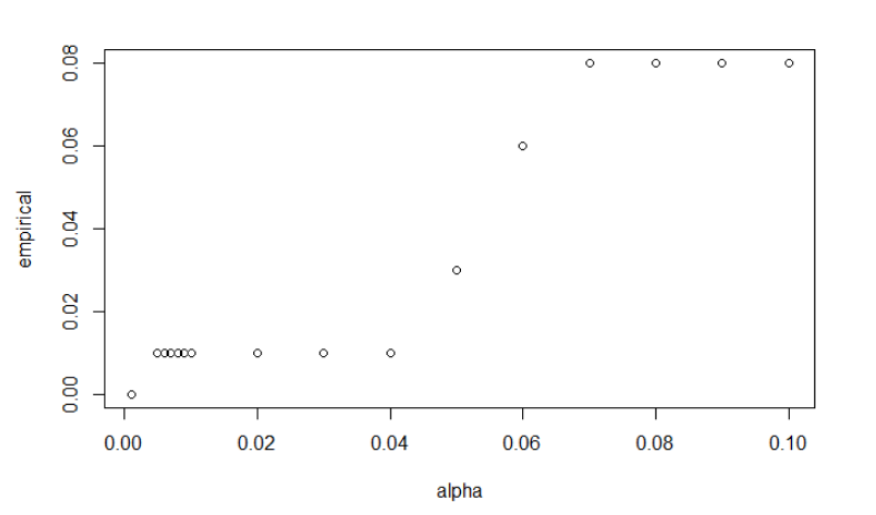
\includegraphics[width=10cm]{Type1_Song1.png}
\caption{Graph of Type 1 error rates for Random Song 1 with 50 observations}
\label{fig: Type 1 Error, Song 1, n=50}
\end{figure}

\begin{figure}[!hb]
\centering
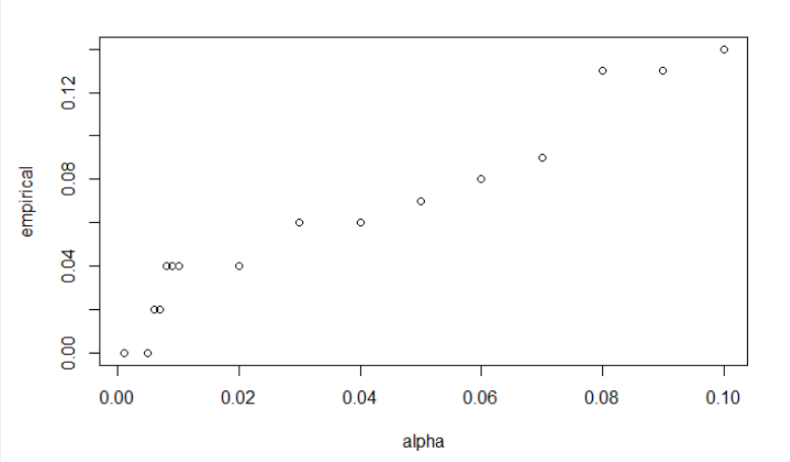
\includegraphics[width=10cm]{Type1_Song2.png}
\caption{Graph of Type 1 error rates for Random Song 2 with 50 observations}
\label{fig: Type 1 Error, Song 2, n=50}
\end{figure}


\subsubsection{Final Power Simulations}
When using the Parametric Bootstrap to return a power, they were generally very low p-values or 0.  The power was always equal to 0 when alpha was set to 0.001 and many of the scenarios gave 0 for every value of alpha.  There were three scenarios that gave actual values which were the both blocks methods and the autoregressive model of order 1 that had 200 notes per song, a probability of missing a note as p=0.1, and $\rho = 0.3$. \\

\begin{tabular}{|c|c|c|c|c|c|}
\hline
\textbf{Type 1 Error Rate Scenario} & $\alpha = 0.001$ &  $\alpha = 0.005$ &  $\alpha = 0.01$ &  $\alpha = 0.05$ &  $\alpha = 0.10$ \\
\hline
Neg. Pair Correlation, n = 200 & 0.00 & 0.00 & 0.00 & 0.00 & 0.00 \\
\hline
Neg. Pair Correlation, n = 600 & 0.00 & 0.00 & 0.00 & 0.00 & 0.00 \\
\hline
Blocks, n = 200 & 0.00 & 0.03 & 0.03 & 0.11 & 0.30 \\
\hline
Blocks, n = 600 & 0.00 & 0.00 & 0.01 & 0.02 & 0.08 \\
\hline
AR(1), p=0.1, $\rho = 0.5$, n = 200 & 0.00 & 0.00 & 0.00 & 0.00 & 0.00 \\
\hline
AR(1), p=0.1, $\rho = 0.5$, n = 600 & 0.00 & 0.00 & 0.00 & 0.00 & 0.00 \\
\hline
AR(1), p=0.1, $\rho = 0.3$, n = 200 & 0.00 & 0.00 & 0.00 & 0.01 & 0.01 \\
\hline
AR(1), p=0.1, $\rho = 0.3$, n = 600 & 0.00 & 0.00 & 0.00 & 0.00 & 0.00 \\
\hline
AR(1), p=0.2, $\rho = 0.5$, n = 200 & 0.00 & 0.00 & 0.00 & 0.00 & 0.00 \\
\hline
AR(1), p=0.2, $\rho = 0.5$, n = 600 & 0.00 & 0.00 & 0.00 & 0.00 & 0.00 \\
\hline
\end{tabular} \\

From the table, it is evident that most of the values obtained are 0 with exceptions for three of the scenarios.  Aside from the table, the graphs also show the large number of occurrences of 0 as a power.  \\

\begin{figure}[!hb]
\centering
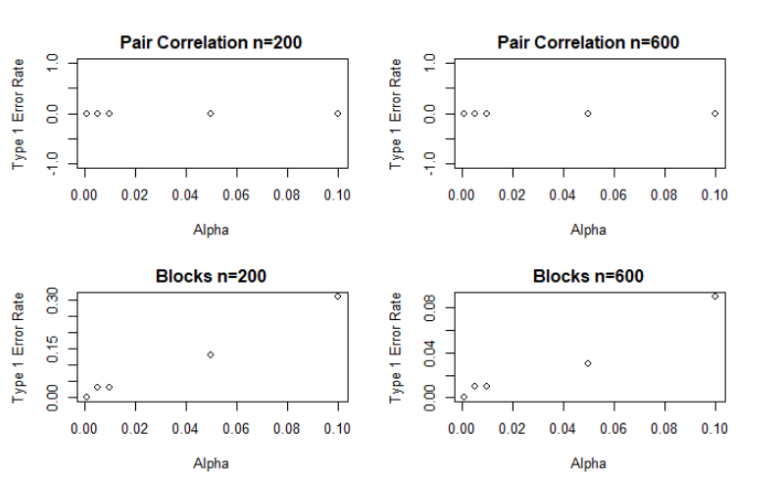
\includegraphics[width=10cm]{PowerGraphs1.png}
\caption{Graph of first four scenarios to calculate the power of a test}
\label{fig: Power Graphs 1}
\end{figure}

\begin{figure}[!hb]
\centering
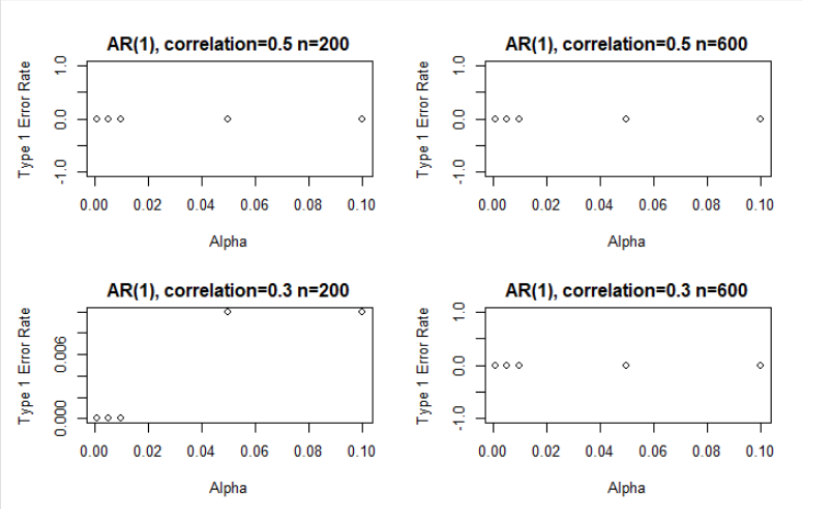
\includegraphics[width=10cm]{PowerGraphs2.png}
\caption{Graph of last four scenarios to calculate the power of a test}
\label{fig: Power Graphs 2}
\end{figure}


\subsection{Permutation Test}
\subsection{Regular Bootstrap}


\section{APPLICATION}
To obtain a p-value for each song, 100 bootstraps were performed to change the 0's and 1's to different orders and sequences.  Previously, 1000 bootstraps were being done, but it was taking a significant amount of time to return a p-value.  The null hypothesis being followed is that the songs are random and the alternative hypothesis is that the songs are not random. 

\subsection{Song 1: "Judith"}

\subsubsection{Parametric Bootstrap}
\begin{tabular}{|c|c|c|}
\hline
\textbf{Method Type} & P-Value \\
\hline
Method 1 & 0 \\
\hline
Runs Test & 0.512 \\ 
\hline
\end{tabular}


\subsubsection{Permutation Tests}
\subsubsection{Regular Bootstrap}

\subsection{Song 2: "Hurts"}

\subsubsection{Parametric Bootstrap}
\begin{tabular}{|c|c|c|}
\hline
\textbf{Method Type} & P-Value \\
\hline
Method 1 & 0  \\
\hline
Runs Test & 0.512 \\ 
\hline
\end{tabular}

\subsection{Song 3: "American Girl"}
\subsubsection{Parametric Bootstrap}

\begin{tabular}{|c|c|}
\hline
\textbf{Method Type} & P-Value \\
\hline
Method 1 & 0.16 \\
\hline
Runs Test & 0.211 \\ 
\hline 
\end{tabular}

\subsection{Song 4: "Funky"}
\subsubsection{Parametric Bootstrap}

\begin{tabular}{|c|c|c|}
\hline
\textbf{Method Type} & P-Value \\
\hline
Method 1 & 0 \\
\hline
Runs Test & 0.08  \\ 
\hline
\end{tabular}

\subsection{Song 5: "Ring of Fire"}
\subsubsection{Parametric Bootstrap}

\begin{tabular}{|c|c|c|}
\hline
\textbf{Method Type} & P-Value  \\
\hline
Method 1 & 2.204 $[e^{-16}]$ \\
\hline
Runs Test & 0.44 \\ 
\hline
\end{tabular}

\subsection{Song 6: "Watchtower"}
\subsubsection{Parametric Bootstrap}

\begin{tabular}{|c|c|c|}
\hline
\textbf{Method Type} & P-Value  \\
\hline
Method 1 & 2.204 $[e^{-16}]$ \\
\hline
Runs Test & 0.66 \\ 
\hline
\end{tabular}
\subsection{Song 7: "Wolf"}
\subsubsection{Parametric Bootstrap}

\begin{tabular}{|c|c|c|}
\hline
\textbf{Method Type} & P-Value  \\
\hline
Method 1 & 2.204 $[e^{-16}]$ \\
\hline
Runs Test & 0.58 \\ 
\hline
\end{tabular}


\section{DISCUSSION/LIMITATIONS/IDEAS FOR FURTHER RESEARCH}

\section{APPENDIX}

\begin{figure}[!hb]
\centering
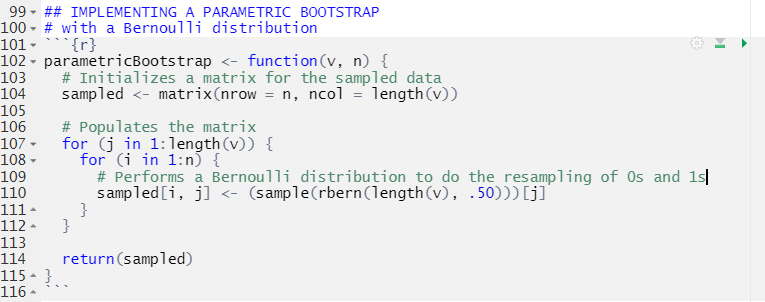
\includegraphics[width=10cm]{ParametricBootstrapCode.png}
\caption{Code to perform a Parametric Resampling on the data given}
\label{fig: Parametric Bootstrap Code}
\end{figure}

\begin{figure}
\centering
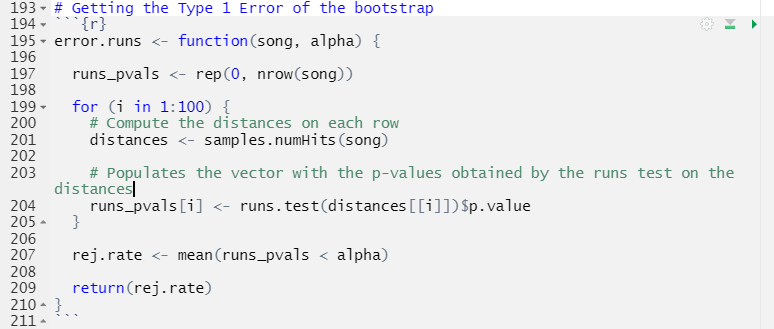
\includegraphics[width=10cm]{Type1ErrCode.png}
\caption{Code to get the Type 1 error of the inputted song}
\label{fig: Type 1 Error Code}
\end{figure}

\begin{figure}
\centering
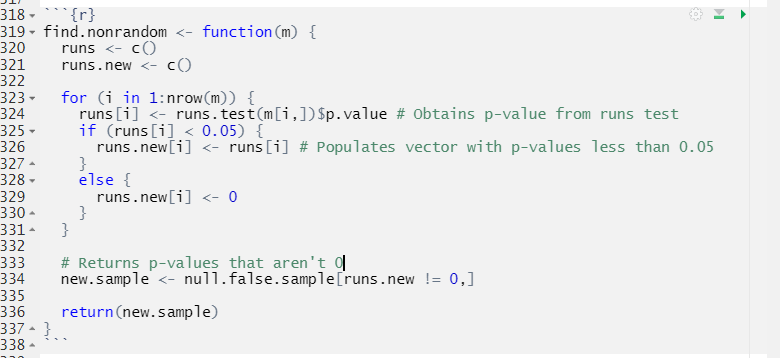
\includegraphics[width=10cm]{FindNonRandomCode.png}
\caption{Code finds the songs that are not random within the matrix}
\label{fig: Find Nonrandom Songs Code}
\end{figure}

\begin{figure}
\centering
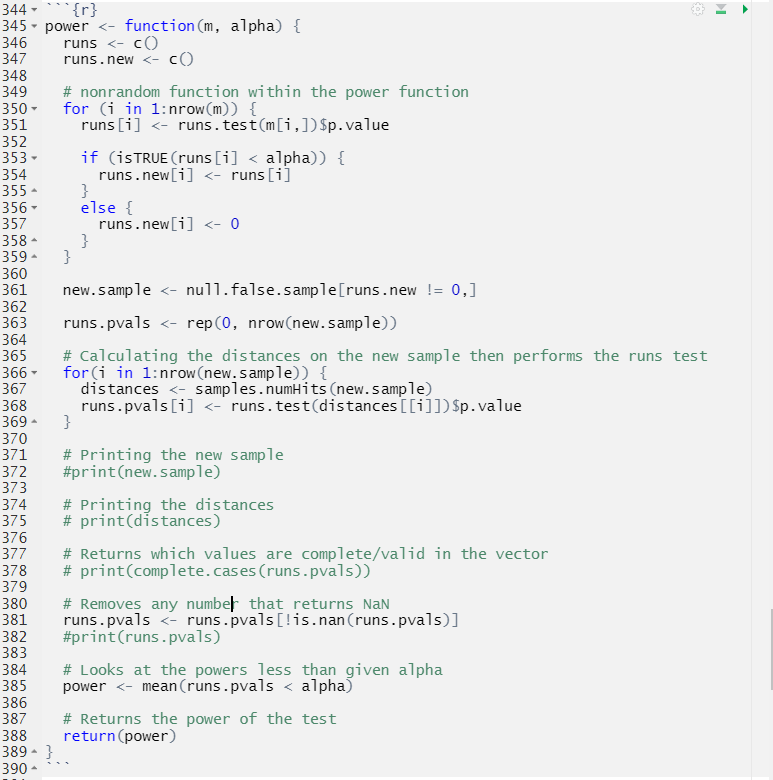
\includegraphics[width=10cm]{PowerCode.png}
\caption{Calculates the power of the test being performed on the song}
\label{fig: Power Code}
\end{figure}


\section{PERSONAL REFLECTIONS}
\subsection{Brianna Cirillo}
\subsection{Samantha Colucci}
\subsection{Shannon Coyle}


\end{document}